\section{Grundlagen des Protokolls}
\label{sec:grundlagen_des_protokolls}

Dieses Kapitel beschreibt die grundlegenden Konzepte und Technologien, die für das Protokoll verwendet werden. Zunächst wird die Peer-to-Peer Funktionalität erläutert, gefolgt von einer Beschreibung des ICE-Protokolls. Anschließend wird die Blockchain-Technologie erläutert, gefolgt von einer Beschreibung der verwendeten Kryptographie.

Peer-to-Peer ist ein dezentrales Kommunikationsmodell, bei dem alle Teilnehmer gleichberechtigt sind und sowohl als Client als auch als Server fungieren können. Im Gegensatz zu einem Client-Server-Modell, bei dem ein zentraler Server die Kommunikation zwischen den Teilnehmern verwaltet, kommunizieren die Teilnehmer in einem Peer-to-Peer-Netzwerk direkt miteinander. Dieses Modell bietet eine Reihe von Vorteilen, wie z.B. eine höhere Skalierbarkeit, da die Last auf mehrere Teilnehmer verteilt wird, und eine höhere Ausfallsicherheit, da das Netzwerk nicht von einem zentralen Server abhängig ist. 
Das Verwenden einer zentralen Instanz kann zu einem Single Point of Failure führen, der das gesamte Netzwerk beeinträchtigen kann, wenn er ausfällt. Doch es hat auch Vorteile, ein zentrales System zu verwenden, da es einfacher ist, die Teilnehmer zu identifizieren, da es eine zentrale Instanz gibt, die die Teilnehmer verwaltet. Dafür sind Peer-to-Peer-Netzwerke schwieriger zu zensieren, da es keine zentrale Instanz gibt, die zensiert werden kann. Ein Nachteil des Peer-to-Peer-Modells ist jedoch, dass es in Abwesenheit eines Servers schwieriger ist, Teilnehmer zu finden oder sie zu verwalten. Dieses Problem kann durch die Verwendung eines strukturierten Peer-to-Peer-Netzwerks gelöst werden, das eine explizite Organisationsstruktur für die Teilnehmer bietet, um die Suche und Verwaltung zu erleichtern \parencite{Luntovskyy_ModRechnernetze}.

\begin{center}
    \captionsetup{type=figure}
    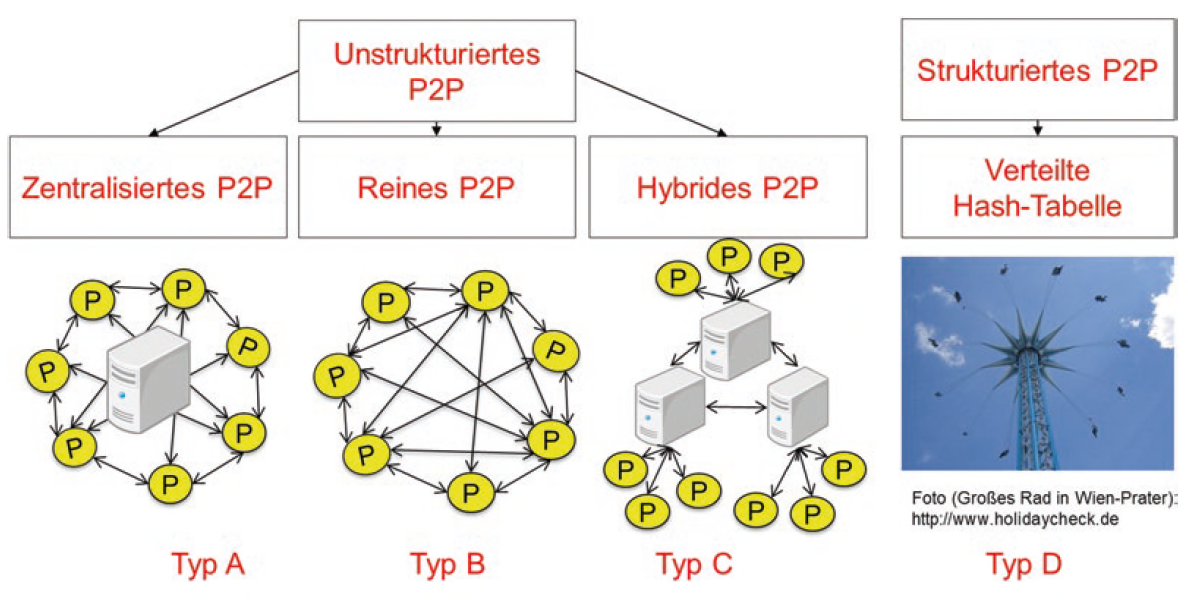
\includegraphics[width=1\linewidth]{images/peer_to_peer_typen.png}
    \captionof{figure}{Typen von Peer-to-Peer-Netzwerken \parencite{Luntovskyy_ModRechnernetze}}
    \label{p2p_typen}
\end{center}

\noindent Unstrukturierte, strukturierte und hybride Peer-to-Peer-Netzwerke sind unterschiedliche Ansätze zur Organisation von Knoten und Ressourcen in dezentralen Netzwerken. Unstrukturierte Netzwerke sind charakterisiert durch ihre fehlende explizite Organisationsstruktur, was eine einfache Konnektivität ermöglicht. Diese Netzwerke sind dynamisch und erlauben es Knoten frei beizutreten oder das Netzwerk zu verlassen, ohne die Gesamtstruktur signifikant zu beeinflussen. Die Suche nach Ressourcen oder Informationen erfolgt oft durch Broadcasts oder zufällige Weiterleitungen, was jedoch zu ineffizienten Suchprozessen führen kann, da keine klare Routing-Struktur vorhanden ist. Ein klassisches Beispiel für ein unstrukturiertes Netzwerk ist das Gnutella-Netzwerk, das sich durch seine dezentrale Natur auszeichnet, jedoch bei der effizienten Ressourcenlokalisierung Schwierigkeiten aufgrund des fehlenden organisierten Routings hat \textcolor{red}{[QUELLE]}.

Strukturierte Peer-to-Peer-Netzwerke hingegen weisen klare Regeln und Algorithmen zur Organisation der Knoten auf. Diese Netzwerke verfügen über eine explizite Organisationsstruktur, sei es eine Ringstruktur, k-bucket basierte Systeme oder andere, die es ermöglichen, effizientes Routing und eine optimierte Ressourcenverwaltung zu erreichen. Durch diese klar definierte Struktur sind strukturierte Netzwerke oft stabiler und bieten eine effizientere Ressourcenlokalisierung im Vergleich zu ihren unstrukturierten Gegenstücken. Allerdings kann diese Stabilität auf Kosten von Flexibilität und Anpassungsfähigkeit gehen, da Änderungen in der Netzwerktopologie oder hohe Dynamik der Knoten schwerer zu handhaben sind \textcolor{red}{[QUELLE]}.

Hybride Peer-to-Peer-Netzwerke versuchen, das Beste aus beiden Welten zu vereinen, indem sie Elemente aus strukturierten und unstrukturierten Ansätzen kombinieren. Diese Netzwerke integrieren Aspekte einer festen Organisationsstruktur für bestimmte Netzwerkbereiche, während andere Bereiche eher unstrukturiert sind. Als Beispiel hierfür kann Napster genannt werden, das eine oder mehrere Nodes dazu verwendet, um die Inhalte innerhalb des Netzwerks zu indizieren und zu verwalten, während der tatsächliche Download des Inhalts über eine direkte Verbindung zwischen den Teilnehmern erfolgt \parencite{Yang_ComparingHybridP2PSystems}.
Ziel ist es, Flexibilität und Effizienz zu optimieren und gleichzeitig eine gewisse Stabilität zu gewährleisten. Diese hybriden Ansätze streben danach, eine ausgewogene Lösung zu bieten, die sowohl die Anforderungen an eine stabile Struktur als auch an eine dynamische und flexible Umgebung erfüllt, je nach den spezifischen Bedürfnissen und Anwendungsfällen \textcolor{red}{[QUELLE]}.

Um die Peer-to-Peer Funktionalität für das Protokoll dieser Arbeit zu gewährleisten, wird ein bereits existierendes Netzwerkprotokoll verwendet. In die engere Auswahl kamen Chord und Kademlia, welche beide lange Gegenstand intensiver Forschung waren, sowohl in der Industrie als auch in der akademischen Welt \parencite[S. 808]{MedranoChavez_ChordKademliaHighChurnScenarios}. 
Das Chord-Protokoll und das Kademlia-Protokoll sind zwei grundlegend verschiedene Ansätze zur Organisation von Peer-to-Peer-Netzwerken. Beide Protokolle sind strukturiert und bieten eine effiziente Ressourcenlokalisierung, aber sie unterscheiden sich in ihrer Routing-Struktur und der Art und Weise, wie sie die Knoteninformationen verwalten.

Chord basiert auf einer Ringstruktur (siehe Abbildung \ref{chord_ring}), bei der die Knoten in einem Ring angeordnet sind und jeder Knoten für einen bestimmten Schlüsselbereich verantwortlich ist. Die Verbindungen zwischen den Knoten sind durch ihren Platz im Ring definiert, wobei jeder Knoten eine Verbindung zu seinem nächsten Nachbarn im Uhrzeigersinn hat. Bei der Suche nach einem bestimmten Schlüssel durchläuft eine Anfrage einen logarithmischen Pfad im Ring, wobei die Knoten auf dem Weg begrenzte Informationen über andere Knoten behalten, um Anfragen weiterzuleiten. Dieses Modell ist recht einfach und effizient für viele Anwendungsfälle, aber es könnte anfällig sein für Engpässe oder längere Suchzeiten, insbesondere wenn das Netzwerk dynamisch ist und sich die Konfiguration häufig ändert.

\begin{center}
    \captionsetup{type=figure}
    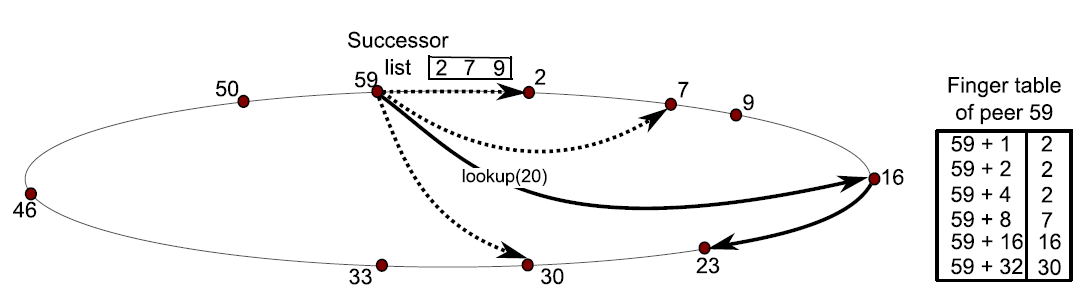
\includegraphics[width=0.9\linewidth]{images/chord_ring.png}
    \captionof{figure}{Visualisierung der Ringstruktur von Chord \parencite{MedranoChavez_ChordKademliaHighChurnScenarios}}
    \label{chord_ring}
\end{center}

\noindent Im Gegensatz dazu verwendet Kademlia eine K-Bucket-Struktur, die in Abbildung \ref{kademlia_tree} zu sehen ist, um eine effiziente Verwaltung von Knoteninformationen zu ermöglichen. Die K-Buckets enthalten eine Liste von Knoten für verschiedene Schlüsselbereiche basierend auf ihrer Nähe, die durch XOR-Distanzen der IDs berechnet wird. Die Verbindungen zwischen den Knoten sind asymmetrisch, und jeder Knoten speichert Informationen über andere Knoten in seinen K-Buckets. Bei der Suche nach einem bestimmten Schlüssel erfolgt das Routing durch die XOR-Entfernung, wodurch die nächsten Knoten für diesen Schlüssel gefunden werden. Dieses Verfahren ermöglicht ebenfalls eine logarithmische Anzahl von Schritten für die Suche und bietet eine robuste Struktur, die gut mit dynamischen Netzwerkänderungen umgehen kann.

\begin{center}
    \captionsetup{type=figure}
    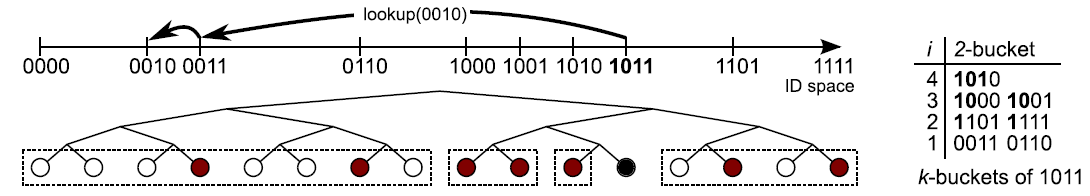
\includegraphics[width=0.9\linewidth]{images/kademlia_tree.png}
    \captionof{figure}{Visualisierung der Baumstruktur von Kademlia \parencite{MedranoChavez_ChordKademliaHighChurnScenarios}}
    \label{kademlia_tree}
\end{center}


\noindent Da bei einem Instant-Messaging-Protokoll häufig Teilnehmer das Netzwerk verlassen und neue Teilnehmer dem Netzwerk beitreten, ist es wichtig, dass das Protokoll mit hoher Fluktuation umgehen kann. Diese Fluktuation von Nodes wird als Churn (engl. Abwanderung) bezeichnet. In einer Studie von Medrano-Chávez et al. \parencite{MedranoChavez_ChordKademliaHighChurnScenarios}, welche im hybriden Journal \textit{Peer-to-Peer Networking and Applications} veröffentlicht wurde, wurde die Leistung von Chord und Kademlia in Bezug auf Netzwerkfluktuation untersucht. Die Ergebnisse zeigen, dass Kademlia bei hoher Fluktuation besser abschneidet als Chord. Aus diesem Grund wird Kademlia in diesem Protokoll als Grundlage für das Auffinden von Teilnehmern und das Routing verwendet.

Um die Problematik mit Firewalls und NAT-Gateways zu lösen, wird das ICE-Protokoll verwendet. ICE ist ein Framework, das mehrere Techniken kombiniert, um eine Verbindung zwischen zwei Endpunkten herzustellen, die sich hinter NATs oder Firewalls befinden. Genaue Details zur Implementierung von ICE folgt in Kapitel \ref{subsec:verbindungsmanagement} \textit{\nameref{subsec:verbindungsmanagement}}.


